
%%% Local Variables:
%%% mode: latex
%%% TeX-master: section03.tex
%%% End:
%%%%%%%%%%%%%%%%%%%%%%%%%%%%%%%%%%%%%%%%%%%%%%%%%%%%%%%%%%%
\section{R简介}
%%%%%%%%%%%%%%%%%%%%%%%%%%%%%%%%%%%%%%%%%%%%%%%%%%%%%%%%%%%%
\subsection{为什么用R}
\begin{frame}{\subsecname}{}

  \begin{columns}
    \begin{column}{.5\textwidth}
      \begin{figure}
        \centering 
\includegraphics[width=\columnwidth]{乾坤大挪移.jpg}
      \end{figure}
    \end{column}

    \begin{column}{.5\textwidth}
      \begin{ornamentblock}
        {吾尝终日而思矣,不如须臾之所学也;吾尝跂而望矣,不如登高之博见也\\
          \rightline{\textemdash《荀子·劝学》}}
      \end{ornamentblock}
      % \curlyframe{工欲善其事,必先利其器\\
      % \rightline{-----《论语·卫灵公》}}
    \end{column}
  \end{columns}
\end{frame}

\begin{frame}[t]{\subsecname}{R的历史}

\begin{itemize}
\item<1-> R诞生于1995年,由新西兰Auckland大学统计学家\emphText{R}obert Gentleman
        和\emphText{R}oss Ihaka开发,而且完全开放源代码,是一款
        基于GNU General Public License(GPL)协议的开源软件;
由于两位开发者的名字都以“R”开头,而且为了向S语言致敬,因此命名为R
\item<2-> R是“所想即所得”工具,其核心是基于S语言设计的R语言,S语言的代码可以不经过
        任何修改就在R中运行,因此R被看做是S语言的非商业化实现  
\end{itemize}

\begin{overlayarea} {\textwidth}{\textheight}
    \begin{figure}\centering
      \captionsetup[subfigure]{labelformat=empty} 
      \subfloat[Ross Ihaka]
      {
\includegraphics[width=0.45\columnwidth]{Ross_Ihaka.png}} \vspace{1pt}
      \subfloat[Robert Gentleman]
      {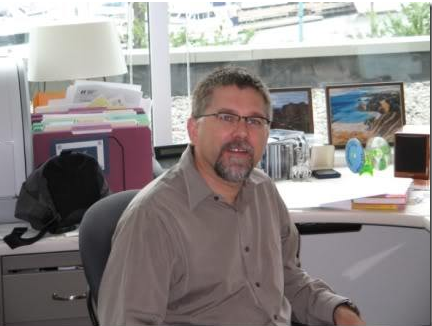
\includegraphics[width=0.4\columnwidth]{Robert_Gentleman.png}} 
    \end{figure}
\end{overlayarea}

\end{frame}

\begin{frame}[t]{\subsecname}{R的优势}
\begin{itemize}
\item<1-> R具备S-Plus几乎所有的优点,而且更加小巧轻便
\item<2-> 开源项目,完全免费,这点是其他统计软件都不具备的
\item<3-> 世界各地有大量研究机构和专业统计人员使用
                 并自愿贡献代码,具有良好的生态系统
\end{itemize}  

\begin{overlayarea}{\textwidth}{\textheight}

\only<1-2>{
  \begin{figure}[ht]
    \centering
    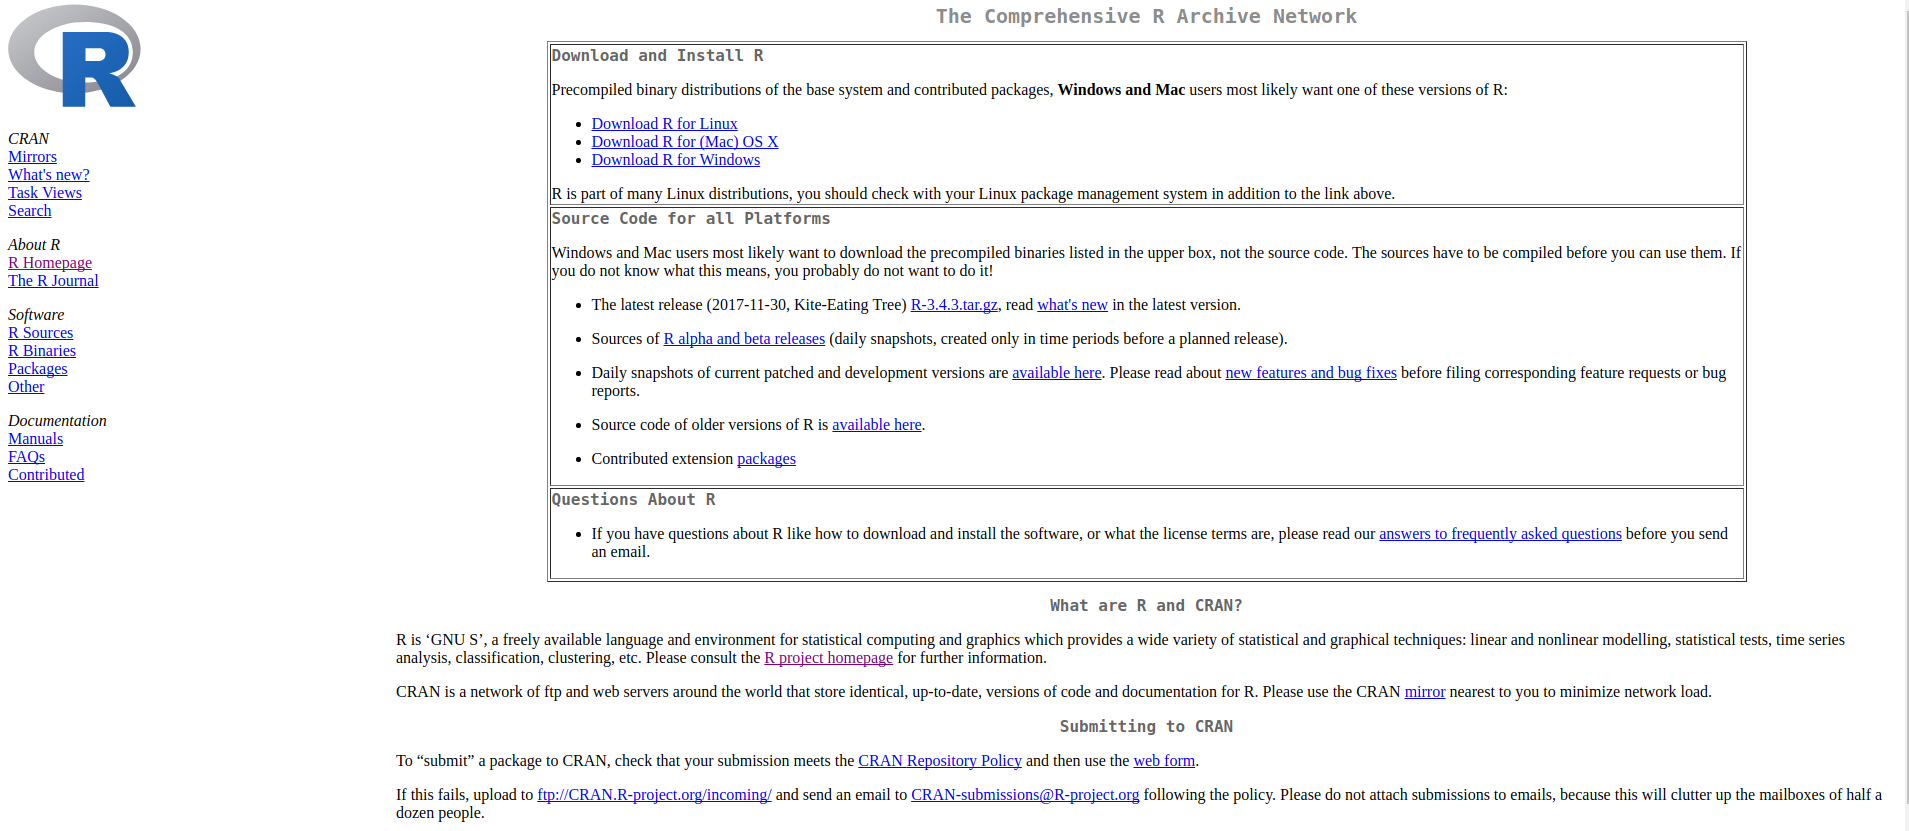
\includegraphics[width=\columnwidth]{CRAN.png}
    \caption{R的官方网站CRAN(https://cran.r-project.org/)}
  \end{figure}}

\only<3->{
  \begin{figure}[ht]
    \centering
    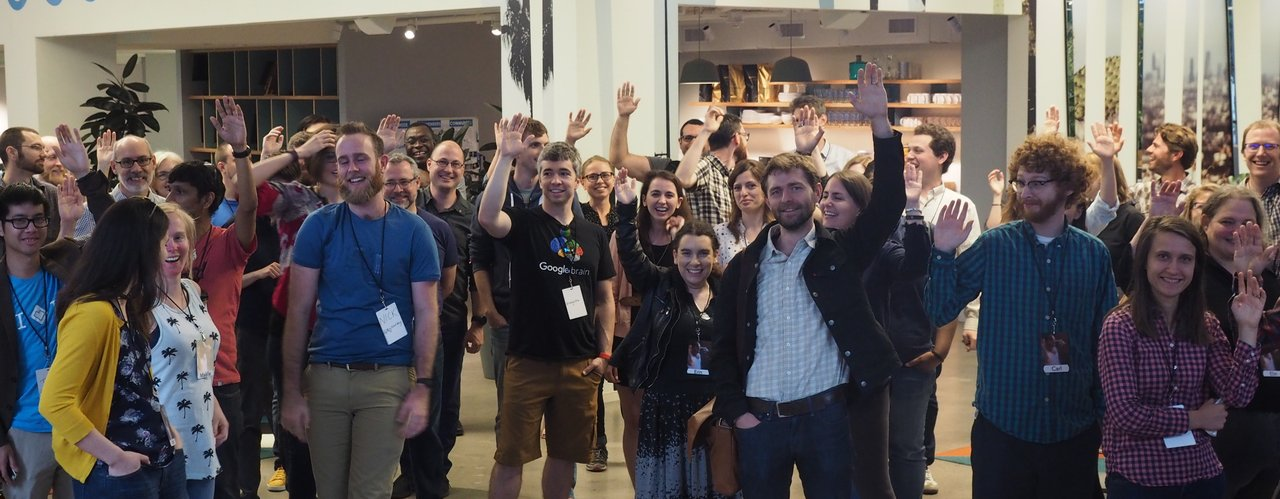
\includegraphics[width=\columnwidth]{R_community.jpg}
    \caption{来自世界各地R的无私贡献者们}
  \end{figure}}
\end{overlayarea}

\end{frame} 

\begin{frame}[t]{\subsecname}{R的优势}
\begin{itemize}
\item<1-> R是高度模块化软件,通过程序包(package)来扩展功能;目前CRAN上
                 的程序包超过12000个,几乎全是来自无偿贡献
\item<2-> R语言语法简单,不需要很高的编程技巧,而且与其他语言具有极好的兼容性
\item<3-> 几乎所有的统计模型都有R语言的实现版本,因此与统计研究前沿相接轨 
\end{itemize}  

\begin{overlayarea}{\textwidth}{\textheight}
\only<1>{
  \begin{figure}[ht]
    \centering
    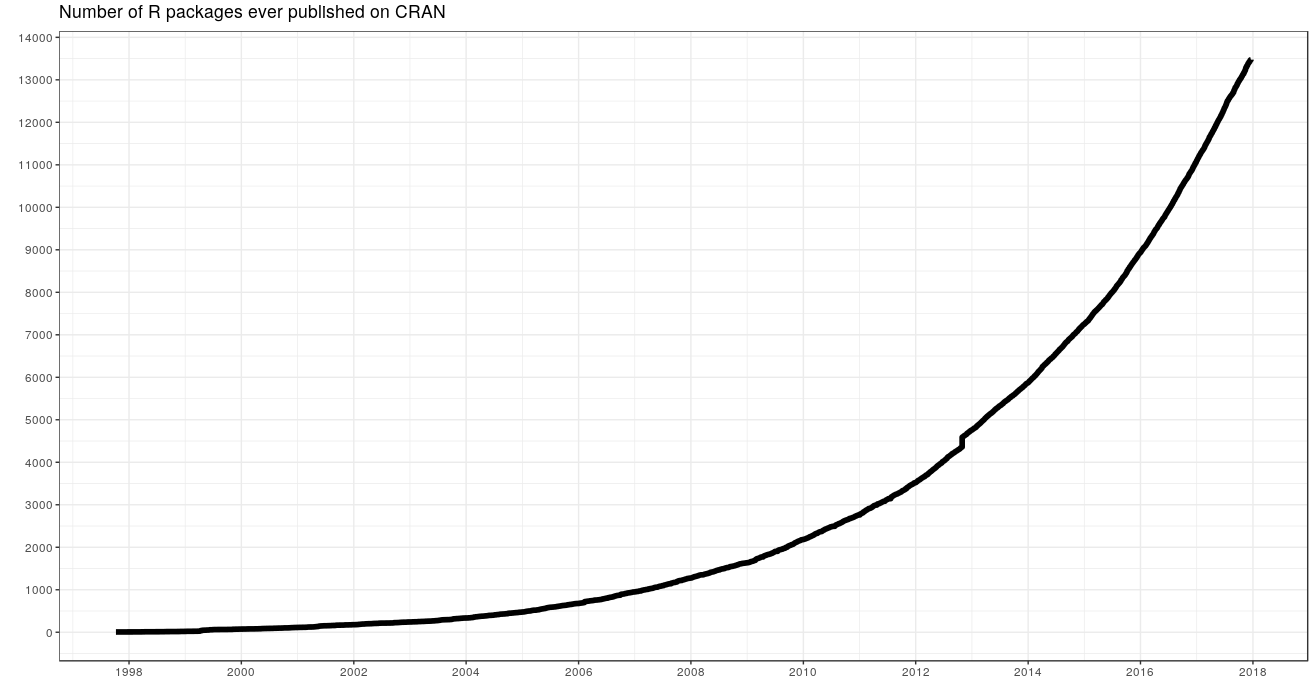
\includegraphics[width=0.7\columnwidth]{number_of_R_packages.png}
    \caption{历年R packages提交的数量统计}
  \end{figure}}

\only<2>{
\begin{block}{R语言的兼容性}
  \begin{itemize}
  \item[\PencilLeftDown] \emphText{内部兼容}:由于R语言本身是解释性语言,
    执行效率较低,因此R的底层函数有很大一部分代码是C语言和Fortran语言编
    写的
  \item[\PencilLeftDown] \emphText{外部兼容}:目前主流的编程语言,例
    如JAVA、c++、python等几乎都有相应的程序库来调用R语言编写的程序,来
    帮助这些编程语言简化统计计算和绘图相关的功能
  \end{itemize}
\end{block}}

\only<3>{
  \begin{figure}
    \centering
    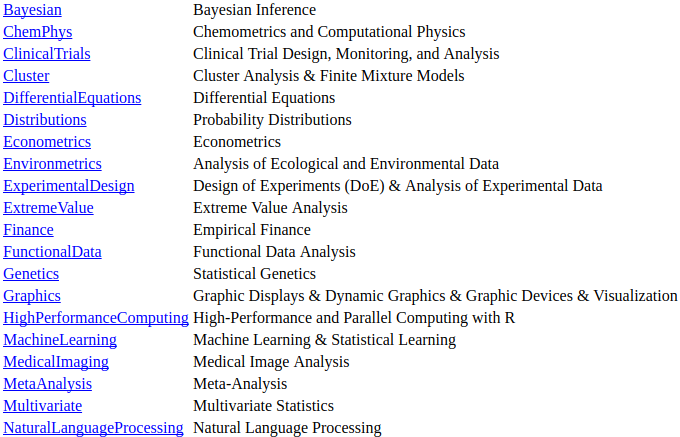
\includegraphics[width=0.55\columnwidth]{CRAN_TASK1.png}
    \caption{R packages的任务分类}
  \end{figure}}

\only<4>{
  \begin{figure}
    \centering
    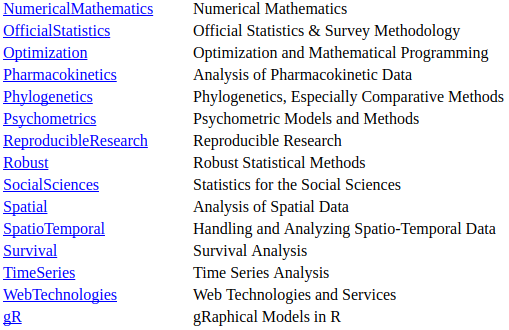
\includegraphics[width=0.55\columnwidth]{CRAN_TASK2.png}
    \caption{R packages的任务分类}
  \end{figure}}
\end{overlayarea}

\end{frame} 

\subsection{基础知识}
\subsubsection{R的工作原理}
\begin{frame}[shrink]{\subsecname}{\subsubsecname}
\begin{itemize}
\item 在R中进行的所有操作都是针对存储在\emphText{内存中的对象}
\item 用户通过输入命令调用函数,\emphText{分析结果可以被直接显示在屏幕上,也可以被存入某个对象或被
写入硬盘}(如图片对象)
\item 因为分析结果本身也是对象,所以它们也能\emphText{被视为数据并能像一般数据那样被处理分析}
\item 数据可以从本地磁盘读取,也可从远程服务器端获得 
\end{itemize} 

\begin{figure}[ht]
  \centering
  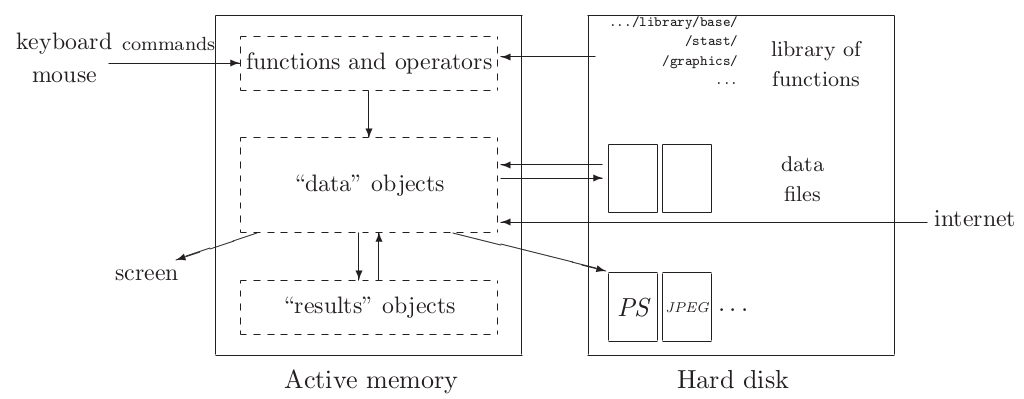
\includegraphics[width=0.9\columnwidth]{R_principle.png}
  \caption{R的工作原理}
\end{figure}
\end{frame}

\subsubsection{安装运行环境}
\begin{frame}[t]{\subsecname}{安装运行环境}
\begin{itemize}
\item R的主安装程序由自愿者进行编译上传,基本上每个在CRAN上可以自由下载,包括windows、linux
                 和mac三大主流平台
\item 安装后的程序界面是一个交互式命令行终端,默认由一个“>”符号表示命令输入和结果
                 输出指示符
\item 在windows有一个简陋的GUI,linux和mac下默认只有CLI终端 
\end{itemize} 

\begin{overlayarea}{\textwidth}{\textheight}
\only<1>{
  \begin{figure}[ht]
    \centering
    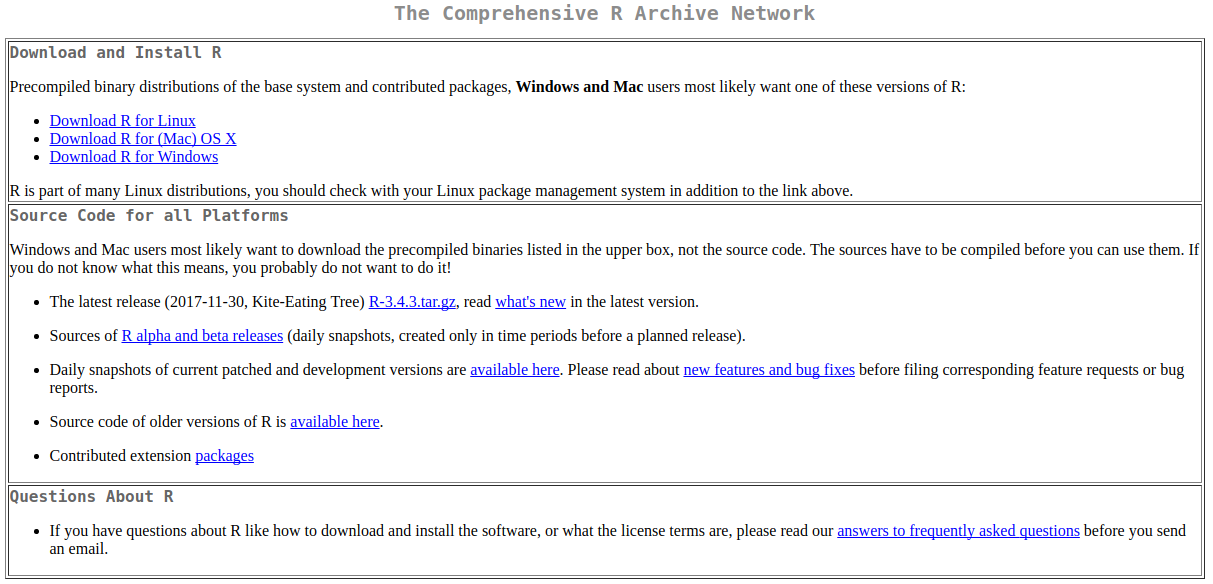
\includegraphics[width=0.8\columnwidth]{R_download.png}
    \caption{R在CRAN的下载界面}
  \end{figure}}

\only<3>{
  \begin{figure}[ht]
    \centering
    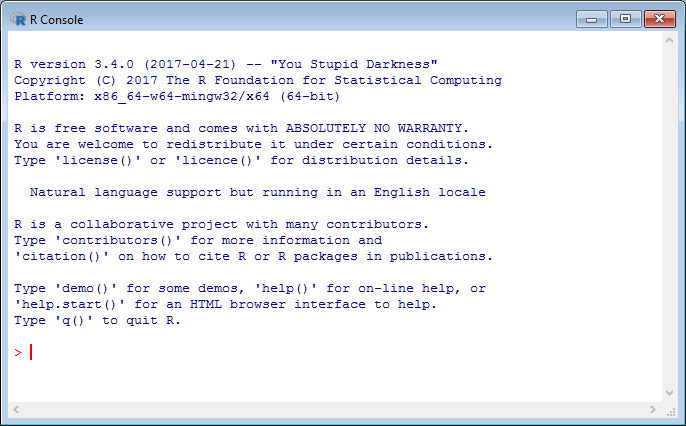
\includegraphics[width=0.6\columnwidth]{R_gui.png}
    \caption{R在windows下的GUI}
  \end{figure}}

\only<4>{
  \begin{figure}[ht]
    \centering
    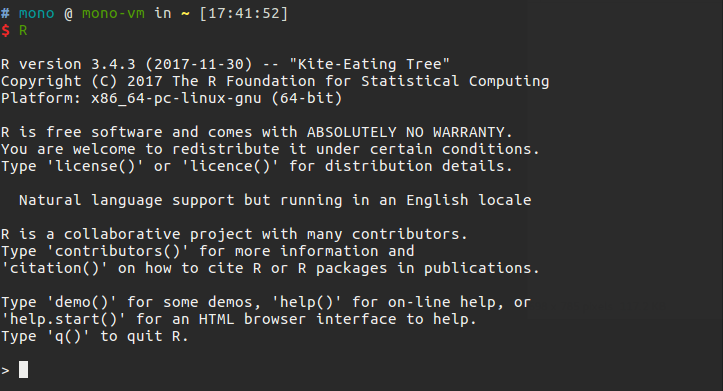
\includegraphics[width=0.7\columnwidth]{R_cli.png}
    \caption{R在linux下的cli终端}
  \end{figure}}
\end{overlayarea}
\end{frame}

\subsubsection{基本操作}
\begin{frame}[t, fragile]{\subsecname}{\subsubsecname}
\begin{itemize}
  \item R的第一种操作就是\emphText{“输入命令$\rightarrow$回车$\rightarrow$输出结果”}这种
             标准的交互式命令行方式  
\end{itemize} 

\begin{overlayarea}{\textwidth}{\textheight}
\begin{onlyenv}<1>
\begin{rcode}
> x = runif(100); y = 0.2*x + 0.1*rnorm(100)
> fit = lm(y ~ x)
> summary(fit)

Call:
lm(formula = y ~ x)

Residuals:
     Min       1Q   Median       3Q      Max 
-0.30665 -0.05002 -0.01135  0.06047  0.24599 

Coefficients:
            Estimate Std. Error t value Pr(>|t|)    
(Intercept)  0.02052    0.01670   1.229    0.222    
x            0.17510    0.03107   5.636 1.67e-07 ***
---
Signif. codes:  0 ‘***’ 0.001 ‘**’ 0.01 ‘*’ 0.05 ‘.’ 0.1 ‘ ’ 1

Residual standard error: 0.08959 on 98 degrees of freedom
Multiple R-squared:  0.2448,    Adjusted R-squared:  0.2371 
F-statistic: 31.77 on 1 and 98 DF,  p-value: 1.671e-07
\end{rcode}
\end{onlyenv}

\begin{onlyenv}<2>
\begin{rcode}
plot(x, y); abline(fit)
\end{rcode}
\begin{figure}
    \centering
    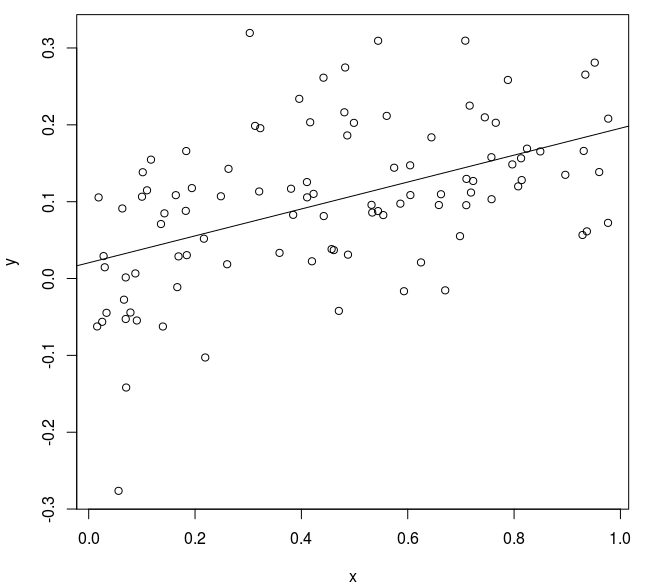
\includegraphics[width=0.55\columnwidth]{R_output.png}
\end{figure}
\end{onlyenv}
\end{overlayarea}
\end{frame}

\begin{frame}[t, fragile]{\subsecname}{\subsubsecname}
\begin{itemize}
\item<1-> 第二种方式是将脚本代码写在文件中,然后一次性运行
\item<2-> 如果代码量很大建议使用第二种方式,因为文件比较容易修改和保存,而且目前
        有专用IDE可以辅助编写R脚本代码  
\end{itemize} 

\begin{overlayarea}{\textwidth}{\textheight}
\only<1>{
  \begin{figure}[ht]
    \centering
    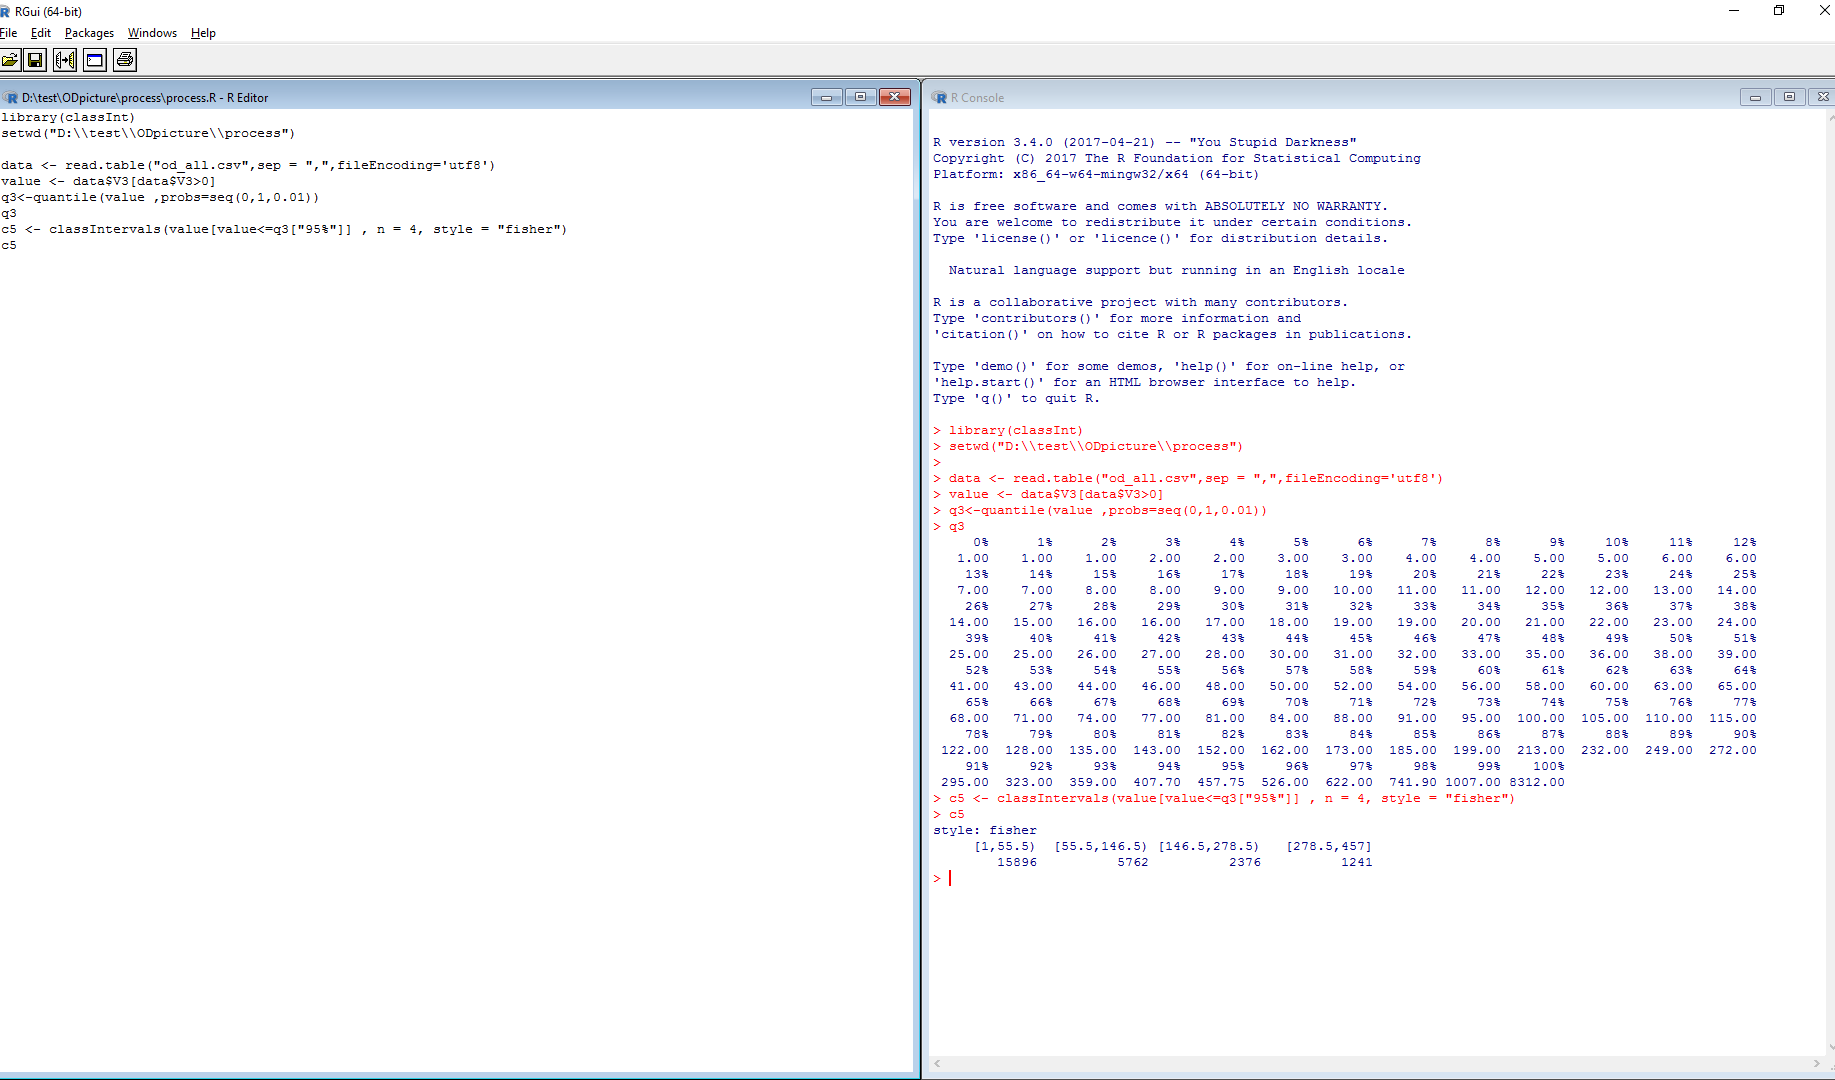
\includegraphics[width=0.8\columnwidth]{R_editor.png}
    \caption{在文本编辑器中编写脚本,然后一次性在终端运行}
  \end{figure}}   

\only<2>{
  \begin{figure}[ht]
    \centering
    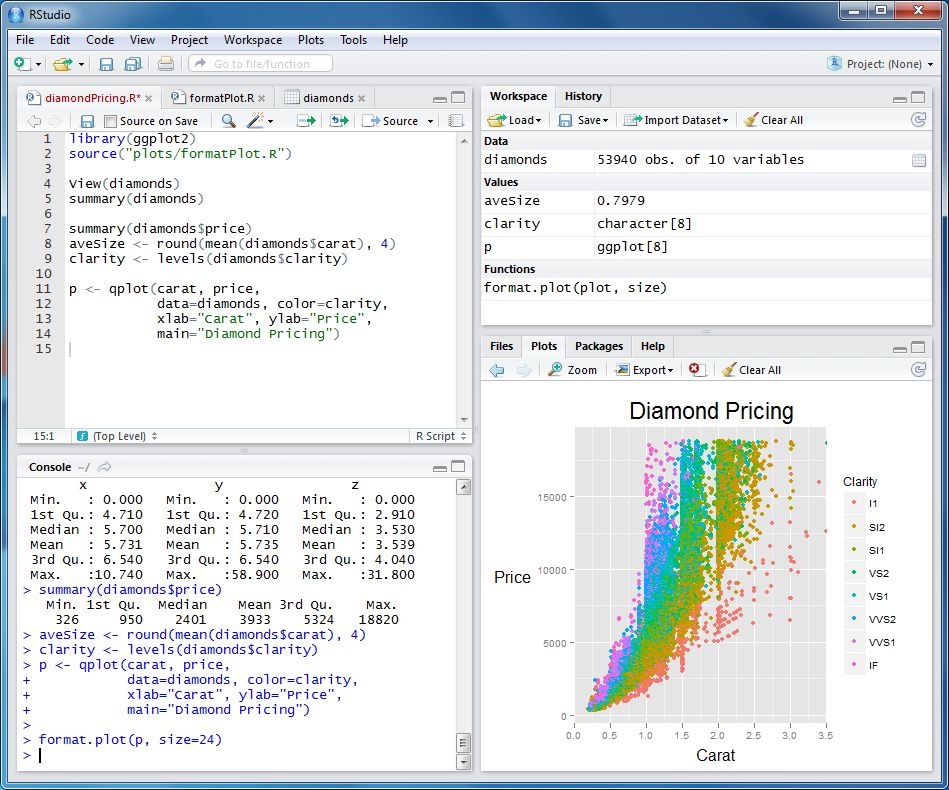
\includegraphics[width=0.6\columnwidth]{RStudio.jpg}
    \caption{\emphText{RStudio}是目前最专业的R IDE,具有大量针对R语言特点设计的功能,
             而且个人桌面版完全开源,可以免费使用}
  \end{figure}}   
\end{overlayarea}
\end{frame}

\subsubsection{程序包}
\begin{frame}[t]{\subsecname}{\subsubsecname}
\begin{itemize}
\item<1-> R的程序包分为\emphText{base包}和\emphText{contrib包}
\item<2-> base包是安装R的时候就自带的,不需要单独安装,
    这类包的质量都非常高,性能稳定
\item<3-> contrib包是自愿者上传的,质量参次不齐;其中质量好
    且用户量大的扩展包有可能会纳入下一个版本的主程序包
\end{itemize}

\begin{overlayarea}{\textwidth}{\textheight}
\only<1>{
  \begin{figure}[h]
    \centering
    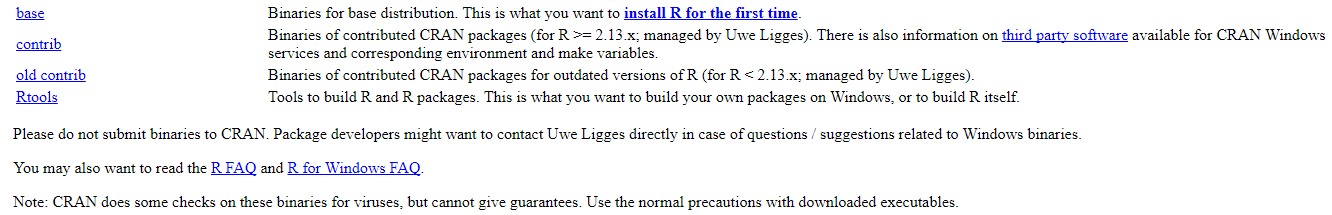
\includegraphics[width=\columnwidth]{R_packages.png}
    \caption{CRAN上下载base包和contrib包}
  \end{figure}}  

\only<2>{
  \begin{table} \centering \small
    \begin{tabular}{|c|c|}
      \toprule
      \rowcolor{LightCyan}
      \textbf{名称} & \textbf{用途}\\\hline
      base & R基础函数包\\\hline
      methods & 用于 R 对象和编程工具的方法和类的定义\\\hline
      datasets & R通用数据集\\\hline
      graphics & 基础统计绘图包 \\\hline
      utils & 通用函数包 \\\hline
      stats & 基础统计计算包 \\\hline
      grDevices & 基础或grid图形设备\\
      \bottomrule
    \end{tabular}
    \caption{常用的base包}
  \end{table}}

\only<3>{
  \begin{table} \centering \small 
    \begin{tabular}{|c|c|}
      \toprule
      \rowcolor{LightCyan}
      \textbf{名称} & \textbf{用途}\\\hline
      cluster & 聚类分析包\\\hline
      maptools & 空间数据读取和处理包\\\hline
      spatstat & 空间点数据分析包\\\hline
      sp & 空间数据基础类包\\\hline
      spdep & 空间自相关模型包\\\hline
      ggplot2 & 基于绘图语法的数据可视化包 \\\hline
      knitr & R文学编程包 \\\hline
      \bottomrule
    \end{tabular}
    \caption{常用的contrib包}
  \end{table}}
\end{overlayarea}
\end{frame}

\begin{frame}[t,fragile]{\subsecname}{\subsubsecname}
\begin{itemize}
\item<1-> base包在R启动之后自动加载,可以直接使用;而contrib包则需要通过library函数调用,如果未安装
               相应包则会报错
\item<2-> 通过\emphTextStep{2-}{install.packages}函数安装contrib包
\end{itemize}

\begin{overlayarea}{\textwidth}{\textheight}
\begin{onlyenv}<1->
\begin{rcode}
> library(sp)
Error in library(sp) : there is no package called ‘sp’
\end{rcode}
\end{onlyenv}

\begin{onlyenv}<2>
\begin{rcode}
> install.packages("sp")
Installing package into ‘/home/mono/Softwares/R/3.4’
(as ‘lib’ is unspecified)
--- Please select a CRAN mirror for use in this session ---
trying URL 'http://mirrors.tuna.tsinghua.edu.cn/CRAN/src/contrib/sp_1.2-6.tar.gz'
Content type 'application/octet-stream' length 1133739 bytes (1.1 MB)
==================================================
downloaded 1.1 MB

* installing *source* package ‘sp’ ...
\end{rcode}
\end{onlyenv}
\end{overlayarea}
\end{frame}

\subsubsection{帮助系统}
\begin{frame}[t,fragile]{\subsecname}{\subsubsecname}
\begin{itemize}
\item<1-> 通过\emphTextStep{1-}{?命令}或者\emphTextStep{1-}{help函数}
               查看程序包中函数的本地帮助文档
\item<2-> 通过\emphTextStep{2-}{help.search函数}在整个帮助系统中进行关键字搜索
\item<3-> \emphTextStep{3-}{find函数}可以根据名称精确查找对象,
               \emphTextStep{3-}{apropos函数}可以根据名称模糊查找对象
\end{itemize}

\begin{overlayarea}{\textwidth}{\textheight}
\begin{onlyenv}<1>
\begin{rcode}
> ?lm
lm               package:stats            R Documentation

Fitting Linear Models

Description:

     ‘lm’ is used to fit linear models.  It can be used to carry out regression, single stratum analysis of variance and analysis of covariance (although ‘aov’ may provide a more convenient interface for these).

Usage:

     lm(formula, data, subset, weights, na.action, method = "qr", model = TRUE, x = FALSE, y = FALSE, qr = TRUE, singular.ok = TRUE, contrasts = NULL, offset, ...)
\end{rcode}
\end{onlyenv}

\begin{onlyenv}<2>
\begin{rcode}
> help.search("data input")
Help files with alias or concept or title matching ‘data input’ using fuzzy matching:


utils::read.DIF         Data Input from Spreadsheet
utils::read.table       Data Input


Type '?PKG::FOO' to inspect entries 'PKG::FOO', or 'TYPE?PKG::FOO' for entries like 'PKG::FOO-TYPE'.
\end{rcode}
\end{onlyenv}

\begin{onlyenv}<3>
\begin{rcode}
> find("lm")
[1] "package:stats"
> appropos("lm")
 [1] "colMeans"        ".colMeans"       "confint.lm"      "contr.helmert"  
 [5] "dummy.coef.lm"   "getAllMethods"   "glm"             "glm.control"    
 [9] "glm.fit"         "KalmanForecast"  "KalmanLike"      "KalmanRun"      
[13] "KalmanSmooth"    "kappa.lm"        "lm"              ".lm.fit"        
[17] "lm.fit"          "lm.influence"    "lm.wfit"         "model.matrix.lm"
[21] "nlm"             "nlminb"          "predict.glm"     "predict.lm"     
[25] "residuals.glm"   "residuals.lm"    "summary.glm"     "summary.lm" 
\end{rcode}
\end{onlyenv}

\end{overlayarea}
\end{frame}

\subsection{数据操作}
\subsubsection{对象(object)}
\begin{frame}[t]{\subsecname}{\subsubsecname}
  \begin{itemize}
  \item R语言中操作的实体在技术上来说就是对象(object) 
  \item 语言中使用对象的好处是可以复用,提升自动化程度
  \item R的所有对象有两个内在属性:类型(mode)和长度(length)
  \end{itemize}

  \begin{columns}
    \begin{column}{.5\textwidth}
      \begin{figure}
        \centering 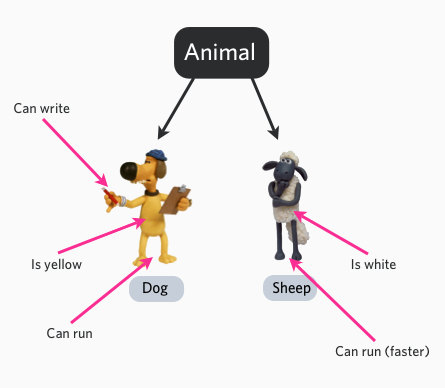
\includegraphics[width=\columnwidth]{object.png}
      \end{figure}
    \end{column}

    \begin{column}{.48\textwidth}
      \begin{ornamentblock}
        \centering
        {在R语言中,几乎任何东西都是对象}
      \end{ornamentblock}
    \end{column}
  \end{columns}
\end{frame}

\subsubsection{数据类型(mode)}
\begin{frame}[t, fragile]{\subsecname}{\subsubsecname}
  \begin{itemize}
  \item 实数型(real):整数(integer)、单精度(single)、双精度(double)
  \item 虚数型(complex):如10+21i
  \item 字符型(character, string):如"hello world"
  \item 逻辑型(logical):TRUE(可以简写成T),FALSE(可以简写成F)
  \item 函数(function)
  \item 表达式(expression)
  \end{itemize}

\begin{overlayarea}{\textwidth}{\textheight}
\begin{rcode}
> x <- 1
> mode(x)
[1] "numeric"
> length(x)
[1] 1
> A <- "Gomphotherium"; compar <- TRUE; z <- 1i
> mode(A); mode(compar); mode(z)
[1] "character"
[1] "logical"
[1] "complex"
# 表达式
> x <- 3; y <- 2.5; z <- 1
> exp1 <- expression(x / (y + exp(z)))
> exp1
expression(x/(y + exp(z)))
> eval(exp1)
[1] 0.5749019
\end{rcode}
\end{overlayarea}
\end{frame}

\subsubsection{数据结构}
\begin{frame}[t]{\subsecname}{\subsubsecname}
  \begin{itemize}
  \item R语言中为了提高数据的使用效率,预定义了专门用于表示数据的对象,也就是数据结构,这些数据结构支撑了R强大的统计分析能力
  \end{itemize}
% \only<1>{
%   \begin{ornamentblock}[userdefinedwidth=0.6\textwidth,align=center]
%         \centering
%         {Everything in R is an object\\
%          Every object in R has a class}
%       \end{ornamentblock}}
  \begin{table} \centering \small
    \begin{tabular}{|c|c|}
      \toprule
      \rowcolor{LightCyan}
      \textbf{数据结构} & \textbf{类型}\\\hline
      向量(vector) & 数值型,字符型,复数型,逻辑型\\\hline
      因子(factor) & 数值型,字符型\\\hline
      数组(array) & 数值型,字符型,复数型,逻辑型\\\hline
      矩阵(matrix) & 数值型,字符型,复数型,逻辑型 \\\hline
      数据框(data.frame) & 数值型,字符型,复数型,逻辑型 \\\hline
      列表(list) & 任意其他类型 \\\hline
      时间序列(ts) & 数值型,字符型,复数型,逻辑型\\
      \bottomrule
    \end{tabular}
    \caption{R基础数据结构}
  \end{table}
\end{frame}

\begin{frame}[t,fragile]{\subsecname}{数据结构}
  \frametitle{}{向量(vector)}
  \begin{itemize}
  \item \emphText{向量是R中最基本的数据单元},向量中的对象类型必须相同
  \item 构建向量常用的函数: rep()、c()、seq()、cbind()、rbind()等
  \item \emphText{向量的下标从1开始},这和其他计算机高级编程语言是不一样的!
  \end{itemize}  

%\begin{overlayarea}{\textwidth}{\textheight}
\begin{rcode}
> x <-1:10; x
[1]  1  2  3  4  5  6  7  8  9 10
> x[3]
[1] 3
> c(7.11, 9.11, 9.19, 1.23)
[1] 7.11 9.11 9.19 1.23
> c("B", "A")
[1] "B" "A"
> rep(1, 10)
[1] 1 1 1 1 1 1 1 1 1 1
> seq(1, 5, 0.5)
[1] 1.0 1.5 2.0 2.5 3.0 3.5 4.0 4.5 5.0
> cbind(0, rbind(1, 1:3))
     [,1] [,2] [,3] [,4]
[1,]    0    1    1    1
[2,]    0    1    2    3
\end{rcode}  
%\end{overlayarea}
\end{frame}

\begin{frame}[t,fragile]{\subsecname}{\subsubsecname}
  \frametitle{}{因子(factor)}
  \begin{itemize}
  \item 因子是对应统计学中的分类数据(categorical data)而设计的
  \item 因子形式上是一个对等长的向量元素进行分类(分组)的向量对象
  \item 因子数据具有水平(level)和标签(label),前者即分类变量的不同取
值,后者即各类取值的名称
  \end{itemize}  

\begin{rcode}
> factor(1:3, labels=c("A", "B", "C"))
[1] A B C
Levels: A B C
> (x = factor(c(1, 2, 3, 1, 1, 3, 2, 3, 3), levels = 1:3,
+   labels = c("g1", "g2", "g3")))
[1] g1 g2 g3 g1 g1 g3 g2 g3 g3
Levels: g1 g2 g3
\end{rcode}  
\end{frame}

\begin{frame}[t,fragile]{\subsecname}{\subsubsecname}
  \frametitle{}{数组(array)和矩阵(matrix)}
  \begin{itemize}
  \item 数组和矩阵是具有维度属性(dimension)的数据结构,
        实质是有附加属性(维数dim)的向量
  \item 矩阵是数组的特例,它的维度为2,用来指定行数和列数
  \end{itemize}  

\begin{rcode}
# 二维矩阵
> matrix(data=5, nr=2, nc=2)
     [,1] [,2]
[1,]    5    5
[2,]    5    5
# 三维数组
> array(1:24, c(3, 4, 2))
, , 1
     [,1] [,2] [,3] [,4]
[1,]    1    4    7   10
[2,]    2    5    8   11
[3,]    3    6    9   12

, , 2
     [,1] [,2] [,3] [,4]
[1,]   13   16   19   22
[2,]   14   17   20   23
[3,]   15   18   21   24
\end{rcode}  
\end{frame}

\begin{frame}[t,fragile]{\subsecname}{\subsubsecname}
  \frametitle{}{列表(list)}
  \begin{itemize}
  \item 列表是一种非常灵活的数据结构,作用是\emphText{生成包含不同类型对象的集合}
  \end{itemize}  

\begin{rcode}
# 创建list
> x <- 1:4; y <- 2:4; L1 <- list(A=x, B=y); L1
$A
[1] 1 2 3 4

$B
[1] 2 3 4
# list元素的索引
> L1[[1]]
[1] 1 2 3 4
> L1["A"]
$A
[1] 1 2 3 4
> L1[["A"]]
[1] 1 2 3 4
> L1$B
[1] 2 3 4
\end{rcode}  
\end{frame}

\begin{frame}[t,fragile]{\subsecname}{\subsubsecname}
  \frametitle{}{数据框(data.frame)}
  \begin{itemize}
  \item 数据框是由许多向量组成的一个二维的对象,主要用于保存建模所需要的数据
  \item 数据框的实质是一个“整齐的”列表,它只要求各列内的数据类型相同,而列之间的可以不同
  \item \emphText{数据框是R中最重要的一种数据结构},大多数数据都是以数据框形式输到R中的
  \end{itemize}  

\begin{rcode}
# 创建数据框
# 数据框中的向量必须有相同的长度,如果其中有一个比其它的短,它将“循环”整数次(以使得其长度与其它向量相同)
> x <- 1:4; M <- c(10, 35); y <- 2:4
> (d <- data.frame(x, M))
  x  M
1 1 10
2 2 35
3 3 10
4 4 35
# data.frame按列进行索引的两种等价的方法
> d$x
[1] 1 2 3 4
> d[["M"]]
[1] 10 35 10 35
> data.frame(x, y)
Error in data.frame(x, y) :
   arguments imply differing number of rows: 4, 3
\end{rcode}  
\end{frame}

\subsubsection{表达式(expression)}
\begin{frame}[t,fragile]{\subsecname}{\subsubsecname}
  \begin{itemize}
  \item 表达式类型对象在R中有着很基础的地位,是R能够解释的字符序列
  \item \emphText{所有有效的R命令都是表达式},表达式分为\emphText{求值表达式和非求值表达式}
  % \item 当命令从被键盘输入后,它就将被R求值,如果是有效命令则会被R解释器执行,因此\emphText{R中
% 有效命令默认都是求值表达式};但是有些情况,需要构造非求值表达式,比如将公式作为函数参数进行传递,
% 或者在图形绘制数学公式等
  \item \emphText{R中有效命令默认都是求值表达式},可以在终端直接输入,
也可以用\emphText{eval函数}执行;而非求值表达式通过\emphText{expression函数}执行
  \end{itemize}  

\begin{overlayarea}{\textwidth}{\textheight}
\begin{onlyenv}<2>
\begin{rcode}
> x <- 3; y <- 2.5; z <- 1
# 创建非求值表达式
> exp1 <- expression(x / (y + exp(z)))
> exp1
expression(x/(y + exp(z)))
# 执行求值表达式
> eval(exp1)
[1] 0.5749019
\end{rcode}  
\end{onlyenv}

\begin{onlyenv}<3>
\vspace{-10pt}
\begin{columns}
  \begin{column}[c]{.5\textwidth} \centering
      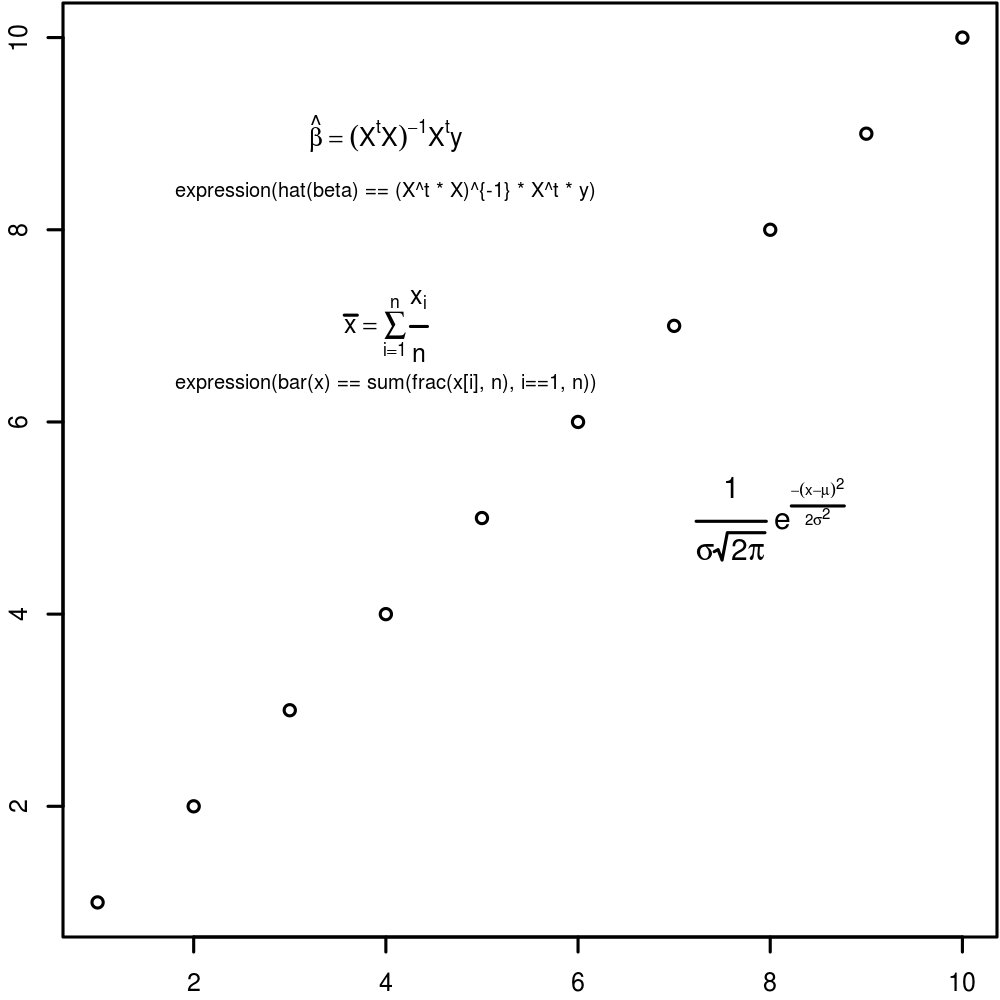
\includegraphics[width=0.8\columnwidth]{expression-example.png}
  \end{column}

  \begin{column}[c]{.5\textwidth}
     \begin{rcode}
     > plot(1:10, 1:10)
     > text(4, 9, expression(hat(beta) == (X^t * X)^{-1} * X^t * y))
     > text(4, 8.4, "expression(hat(beta) == (X^t * X)^{-1} * X^t * y)", cex = .8)
     > text(4, 7, expression(bar(x) == sum(frac(x[i], n), i==1, n)))
     > text(4, 6.4, "expression(bar(x) == sum(frac(x[i], n), i==1, n))", cex = .8)
     > text(8, 5, expression(paste(frac(1, sigma*sqrt(2*pi)), " ", plain(e)^{frac(-(x-mu)^2, 2*sigma^2)})), cex = 1.2)
\end{rcode}  
  \end{column}
\end{columns}
\end{onlyenv}
\end{overlayarea}
\end{frame}

\subsubsection{数据输入输出}
\begin{frame}[t,fragile]{\subsecname}{\subsubsecname}
\begin{itemize}
\item<1-> R的数据可以按照数据结构手动输入,也可以通过读取外部文件自动输入
\item<2-> R base包提供了文本文件(ASCII)的读取函数:\emphTextStep{2-}{read.table}、
                     \emphTextStep{2-}{scan}和\emphTextStep{2-}{read.fwf}等
\item<3-> R base包也提供了文本文件(ASCII)的输出函数:\emphTextStep{2-}{write.table}
\item<4-> 另外,\emphTextStep{4-}{图形作为对象也可以输出},这将在后面会专门介绍
\end{itemize}

\begin{overlayarea}{\textwidth}{\textheight}
\begin{onlyenv}<2>
%\begin{minted}{R}
\begin{rcode}
# 从外部读取data.dat文件,并且将数据赋给一个名为mydata的对象,这里mydata是一个data.frame数据结构
> mydata <- read.table("data.dat")

# read.table的参数
read.table(file, header = FALSE, sep = "", quote = "\"’", dec = ".", row.names, col.names, as.is = FALSE, na.strings = "NA",colClasses = NA, nrows = -1,skip = 0, check.names = TRUE, fill =!blank.lines.skip,strip.white = FALSE, blank.lines.skip = TRUE,comment.char = "#")
\end{rcode}
%\end{rcode}
\end{onlyenv}

\begin{onlyenv}<3>
\begin{rcode}
# 函数write.table可以在文件中写入一个对象,一般是写一个数据框,也可以是其它类型的对象
write.table(x, file = "", append = FALSE, quote = TRUE, sep = " ", eol = "\n", na = "NA", dec = ".", row.names = TRUE, col.names = TRUE, qmethod = c("escape", "double"))
\end{rcode}
\end{onlyenv}

\end{overlayarea}
\end{frame}

\subsection{程序控制}
\begin{frame}{\subsecname}{}
  \begin{itemize}
  \item<1-> if (条件) {表达式}
  \item<1-> if (条件) {表达式} else {表达式}
  \item<1-> if...else if...else if... else...
  \item<1-> ifelse (条件, yes, no)
  \item<2-> for (变量 in 向量) {表达式}
  \item<2-> while (条件) {表达式} 
  \end{itemize}

\onslide<3>{
\begin{badbox}{}
循环的编程模式在R语言中效率很低,尽量避免使用,应该尽量使用基于列表的操作模式!
\end{badbox}} 
\end{frame}

\subsection{函数}
\begin{frame}[t,fragile]{\subsecname}{}
\begin{itemize}
  \item R语言中可以定义函数,以便编程中可以以不同的参数值重复使用同一段代码
  \item 定义函数:\emphText{function(arglist) expr return(value)};
其中arglist是参数列表,expr是函数的主体,return()用来返回函数值
  \item \emphText{函数是R中用于黑箱操作的重要实体}
  \item<2-> R函数的参数除了允许传递常规变量类型之外,
还\emphText{允许以匿名函数的形式将函数作为参数进行传递}
\end{itemize}  

\begin{onlyenv}<1>
\begin{rcode}
# 定义峰度函数kurtosis,该函数有两个参数,数据向量x和是否删除缺失值na.rm,后者有默认值FALSE
> kurtosis = function(x, na.rm = FALSE) {
    if (na.rm)
      x = x[!is.na(x)]
    return(sum((x - mean(x))^4)/(length(x) * var(x)^2) - 3)
  }
> # 引用函数
> kurtosis(runif(100))
[1] -1.36086
\end{rcode}  
\end{onlyenv}

\begin{onlyenv}<2>
\begin{rcode}
# xyplot函数的panel参数传递是一个匿名函数
xyplot(Murder ~ Population | state.region, data = states,
       groups = state.name,
       |colorbox{green}{panel = function(x, y, subscripts, groups)}| {
           ltext(x = x, y = y, labels = groups[subscripts], cex=1,
                 fontfamily = "HersheySans")
       })
\end{rcode}  
\end{onlyenv}
\end{frame}

\subsection{公式}
\begin{frame}[t]{\subsecname}{}
\begin{itemize}
\item<1-> 公式是R中用于统计建模的重要元素,表示统计模型中变量之间的关系,其基本形式是
\emphText{$y \sim mode$};
其中\emphText{y是响应变量},\emphText{mode是一些元素项的集合}而且要为其中一些项估计参数
\item<2-> 元素项通过一些有特殊涵义的运算符连接
\end{itemize} 

\only<2>{
\begin{table} \centering \scriptsize
  \begin{tabular}{|m{0.1\columnwidth}|m{0.8\columnwidth}|}
    \toprule
    \rowcolor{LightCyan}
%     \multicolumn{1}{|>{\centering\arraybackslash}m{0.1\columnwidth}|}{运算符}& 
% \multicolumn{1}{|>{\centering\arraybackslash}m{0.8\columnwidth}|}{含义}\\\hline
 %   \thbf{运算符} & \thbf{含义} \\\hline
\multicolumn{1}{|c|}{\textbf{运算符}} & \multicolumn{1}{c|}{\textbf{含义}} \\\hline
    a+b & a和b的相加效应,例如$y\sim x_1+x_2$表示线性模型$y=\beta_1x_1+\beta_2x_2+\alpha$\\\hline
    X & 如果X是一个矩阵, 这将反映各列的相加效应,即
$X[,1]+X[,2]+...+X[,ncol(X)]$; 还可以通过索引向量
选择特定列进行分析,如$X[,2:4]$\\\hline
    a:b & a和b的交互效应\\\hline
    a*b & 相加和交互效应,等价于a+b+a:b \\\hline
    \^{}n & 包含所有的直到n阶的交互作用,例如$(a+b+c)^2$等价于$a+b+c+a:b+a:c+b:c$ \\\hline
    b \%in\% a & b和a的嵌套分类设计,等价于a+a:b,或者a/b\\\hline
    -b & 去掉因子b的影响, 如:$(a+b+c)^2-a:b$等价于$a+b+c+a:c+b:c$\\\hline
    -1 & $y\sim x-1$表示通过原点的线性回归,等价于$y\sim x+0$或者$0+y\sim x$\\\hline
    1 & $y\sim 1$拟合一个没有因子影响的模型(仅仅是截距)\\\hline
    offset(...) & 向模型中增加一个影响因子但不估计任何参数,例如offset(3*x)\\
    \bottomrule
  \end{tabular}
\end{table}}
\end{frame}

\subsection{面向对象编程}
\begin{frame}[t]{\subsecname}{}
\begin{itemize}
\item \emphText{R语言中支持面向对象(Object-Oriented, OO)编程来提高代码的使用率},从而实现具体功能的扩展和模块化
  \item R语言作为一种统计编程语言,需要用到OO的场景主要有以下两类:
  \begin{itemize}
     \item[\PencilLeftDown] 当需要用一种新的类型来表示数据,该类型与
   已有的数据类型有区别的时候
     \item[\PencilLeftDown] 当需要一个新的函数,该函数可以根据不同的
参数类型做出不同的反应的时候
  \end{itemize}
\item R语言中有四种OO的实现系统:\emphText{S3、S4、RC(R5)和R6}
\end{itemize}  
\end{frame} 

\begin{frame}[t,fragile]{\subsecname}{S3系统}
  \begin{itemize}
  \item S3是R语言的第一种也是最简单的一种OO系统,也是\emphText{CRAN程序包中最常用的一种OO系统}
  \item S3系统中方法(method)是属于函数而不是属于类,这种函数称为\emphText{泛型函数}(generic function)
  \item 泛型函数的形式是\emphText{generic.class()},其实质是根据传入函数的第一个参数的类去调用相应的“子函数”
  \end{itemize}  

  %\begin{overlayarea}{\textwidth}{\textheight}
\begin{rcode}
> library(pryr) # 调用pryr程序包检测某个方法是否是S3系统
> df <- data.frame(x = 1:10, y = letters[1:10])
> otype(df)    # data.frame是一个S3方法
[1] "S3"
# 调用methods()来查看属于某个泛型的所有方法
> methods("mean")
[1] mean.Date   mean.default    mean.difftime   mean.POSIXct    mean.POSIXlt
# 根据传入函数的第一个参数的类去调用相应的“子函数”
> (today <- Sys.Date())
[1] "2018-01-18"
> tenweeks <- seq(today, length.out=10, by="1 week")
> class(tenweeks)
[1] "Date"
> mean(tenweeks) # 这里调用的实际上是mean.Date
[1] "2018-02-18" 
\end{rcode}  
  %\end{overlayarea}
\end{frame}

\subsubsection{S3系统}
\begin{frame}[t,fragile]{\subsecname}{\subsubsecname}
  \begin{itemize}
  \item<1-> 创建S3对象最简单的方法是给一个变量增加\emphText{class属性};也可以通过\emphText{structure()}函数创建
  \item<2-> 使用\emphText{UseMethod()}函数定义S3型泛型函数
  \item<3-> 通过\emphText{NextMethod()}函数实现继承
  \end{itemize}  

\begin{overlayarea}{\textwidth}{0.5\textheight}
\begin{onlyenv}<1>
\begin{rcode}
# 通过给变量增加class属性来创建S3型对象
> x <- 1; attr(x,'class') <- 'foo'
> x
[1] 1
attr(,"class")
[1] "foo"
> otype(x)
[1] "S3"
# 通过structure函数来创建S3型对象
> y <- structure(2, class='foo')
> y
[1] 2
attr(,"class")
[1] "foo"
> otype(y)
[1] "S3"
\end{rcode}  
\end{onlyenv}

\begin{onlyenv}<2>
\begin{rcode}
# 用UseMethod定义S3泛型函数
> teacher <- function(x,...) UseMethod("teacher")
# 定义了三个teacher的内部函数
> teacher.lecture <- function(x) print("上课")
> teacher.assignment <- function(x) print("布置作业")
> teacher.default <- function(x) print("你不是老师")
# 定义一个S3对象a,其class是lecture
> a <- structure('A', class='lecture')
# teacher泛型函数根据传入的类调取teacher.lecture()函数
> teacher(a) 
[1] "上课"
# 默认泛型函数
> teacher()
[1] "你不是老师"
\end{rcode}  
\end{onlyenv}

\begin{onlyenv}<3>
\begin{rcode}
# 定义一个S3泛型函数node
> node <- function(x) UseMethod('node', x)
# 定义node的内部函数,其中son函数通过NextMethod()指向father
> node.default <- function(x) "Default node"
> node.father <- function(x) c("father")
> node.son <- function(x) c("son", NextMethod())
# 定义对象n有两个class,调用node函数会先执行son函数,再执行father函数,模拟了子函数调用父函数的过程
> n <- structure(1, class = c("son", "father"))
> node(n)
[1] "son"    "father"
\end{rcode}
\end{onlyenv}

\begin{onlyenv}<4>
\begin{badbox}{S3系统的缺点}
\begin{itemize}
\item[\PencilLeftDown] S3系统并不是真正的OO,只是通过函数来模拟OO
\item[\PencilLeftDown] S3系统使用简单,但是很难处理复杂的对象关系
\item[\PencilLeftDown] S3系统的内部函数并没有真正封装,可以绕过泛型函数检查直接被调用
\item[\PencilLeftDown] S3系统的class属性可以被任意设置,没有检查机制
\end{itemize}
\end{badbox}
\end{onlyenv}
\end{overlayarea}
\end{frame}

\subsubsection{S4系统}
\begin{frame}[c,fragile]{\subsecname}{\subsubsecname}
  \begin{itemize}
  \item<1-> 相比S3系统,S4系统有更明确和严谨的OO系统特征
  \item<2-> S4有专门的类定义函数\emphText{setClass()}和类的实例化函数\emphText{new()}
  \item<3-> 对象类型检查函数\emphText{setValidity()}
  \item<4-> S4泛型函数实现了方法定义和实现的分离,通过\emphText{setGeneric()}函数定义接口,
    \emphText{setMethod()}函数定义实现方法;\emphText{standardGeneric}定义泛型函数,
类似S3中的UseMethod
  \end{itemize}  

\begin{overlayarea}{\textwidth}{\textheight}
\begin{onlyenv}<2>
\begin{rcode}
# 定义S4类person以及person的子类son
> setClass('person',slots=list(name="character",age="numeric"))
> setClass("son", slots=list(father="person",mother="person"),contains="person")
# 实例化对象
> father <- new("person",name="F",age=44)
> mother <- new("person",name="M",age=42)
> son <- new("son",name="S",age=16,father=father,mother=mother)
# 查看son对象的属性
> son@father
An object of class "person"
Slot "name":
[1] "F"

Slot "age":
[1] 44
\end{rcode}  
\end{onlyenv}

\begin{onlyenv}<3>
\begin{rcode}
# 定义S4类person
> setClass('person',slots=list(name="character",age="numeric"))
# 传入错误的age类型
> bad <- new("person",name="bad",age="aaa")
Error in validObject(.Object) : 
  invalid class “person” object: invalid object for slot "age" in class "person": got class "character", should be or extend class "numeric"
# 设置age属性的非负检查
> setValidity("person",function(object){
+    if(object@age <=0) stop("Age is negative.")
+ })
# 传入age属性小于0时会报错
> bad2 <- new("person",name="bad",age=-1)
Error in validityMethod(object) : Age is negative.
\end{rcode}
\end{onlyenv}

\begin{onlyenv}<4>
\begin{rcode}
# 定义person类,slots参数定义类的属性
> setClass('person',slots=list(name="character",age="numeric"))
# 定义泛型函数work,即接口
> setGeneric("work",function(obj) standardGeneric("work"))
[1] "work"
# 定义work的实现函数,并指定参数类型为person
> setMethod("work",signature(obj="person"),function(obj) cat(obj@name, "is working"))
[1] "work"
# 创建person类型对象a,并将其传入work函数
> a <- new("person",name="Conan",age=16)
> work(a)
Conan is working
\end{rcode}  
\end{onlyenv}
\end{overlayarea}
\end{frame}

\subsubsection{RC和R6系统}
\begin{frame}[t,fragile]{\subsecname}{\subsubsecname}
  \begin{itemize}
  \item<1-> RC(Reference classes),又称为R5,是从2.12版本引入的新一代OO系统
  \item<2-> \emphText{RC系统的方法是在类中定义的},而不是通过泛型函数
  \item<2-> RC系统依赖于S4系统,是对OO的进一步封装,已经非常趋于主流编程语言中的OO实现
  \item<3-> R6是一个\emphTextStep{3}{完全独立的R程序包},类似RC但不依赖于S4系统 
  \end{itemize}  

\begin{overlayarea}{\textwidth}{\textheight}
\begin{onlyenv}<2>
\begin{rcode}
# 定义一个RC类,方法包括在定义中
> user<-setRefClass("user",
+      fields=list(name="character",favorite="vector"), 
+      methods=list(                                                      
+             addFavorite=function(x){
+                 favorite<<-c(favorite,x)},
+             delFavorite=function(x){
+                 favorite<<-favorite[-which(favorite==x)]}))
# 实例化一个u对象
> u <- user$new(name="u",favorite=c('movie','football'))
# 操作方法
> u$addFavorite('shopping')
> u$favorite
[1] "movie"    "football" "shopping"
\end{rcode}  
\end{onlyenv}
\end{overlayarea}
\end{frame}